\documentclass[12pt, twoside]{article}
\usepackage[letterpaper, margin=1in, headsep=0.5in]{geometry}
\usepackage[english]{babel}
\usepackage[utf8]{inputenc}
\usepackage{amsmath}
\usepackage{amsfonts}
\usepackage{amssymb}
\usepackage{tikz}
\usetikzlibrary{quotes, angles}
\usepackage{graphicx}
%\usepackage{pgfplots}
%\pgfplotsset{width=10cm,compat=1.9}
%\usepgfplotslibrary{statistics}
%\usepackage{pgfplotstable}
%\usepackage{tkz-fct}
%\usepackage{venndiagram}

\usepackage{fancyhdr}
\pagestyle{fancy}
\fancyhf{}
\renewcommand{\headrulewidth}{0pt} % disable the underline of the header

\fancyhead[RE]{\thepage}
\fancyhead[RO]{\thepage \\ Name: \hspace{3cm}}
\fancyhead[L]{BECA / Dr. Huson / Geometry 10th Grade\\* Unit 3: Volume and angle bisectors \\ 
2 October 2019}

\begin{document}
\subsubsection*{3.1 Do Now: Angle terminology and notation}
  \begin{enumerate}

  \item As shown below, two lines intersect making four angles: $\angle 1$, $\angle 2$, $\angle 3$, and $\angle 4$.
    \begin{center}
    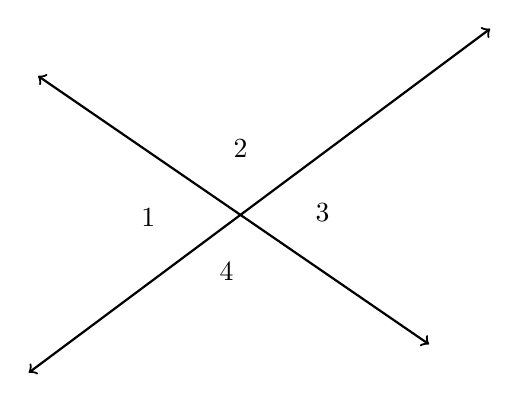
\begin{tikzpicture}[scale=0.7, rotate=20]
      \draw [<->, thick] (0,-1.5)--(10,1.5);
      \draw [<->, thick] (2,3.5)--(7,-3.5);
      \node at (3,.4){1};
      \node at (6,-.6){3};
      \node at (5,1){2};
      \node at (4,-1){4};
      %\draw [fill] (0,0) circle [radius=0.05] node[below]{$P$};
      %\draw [fill] (6,0) circle [radius=0.05] node[below]{$R$};
      %\draw [fill] (3,0) circle [radius=0.05] node[below]{$Q$};
    \end{tikzpicture}
    \end{center}
    \begin{enumerate}
    \item Which angle is opposite $\angle 1$? \rule{4cm}{0.15mm} \bigskip
    \item Name an angle that is adjacent to $\angle 4$. \rule{4cm}{0.15mm} \bigskip
    \item True or false, $\angle 2$ and $\angle 4$ are vertical angles. \rule{3cm}{0.15mm}
  \end{enumerate}

  \item Measure the required angles of the diagram below and answer the questions. \vspace{0.25cm}
  \begin{enumerate}
    \item  $m \angle AOB = $ \rule{2.5cm}{0.15mm} \hspace{0.5cm} $m \angle BOC = $ \rule{2.5cm}{0.15mm} \hspace{0.5cm} $m \angle DOE = $ \rule{2.5cm}{0.15mm}\bigskip
    \item Name an angle that is supplementary to $\angle AOB$: \rule{4cm}{0.15mm} \bigskip
    \item Name an angle that is complementary to $\angle DOE$: \rule{4cm}{0.15mm}
  \end{enumerate}
  \vspace{1cm}
  \begin{center}
  \begin{tikzpicture}[scale=1.3, rotate=-20]
    \draw [<->, thick] (-55:3)--(0,0)--(125:4);
    \draw [<->, thick] (-5,0)--(5,0);
    \draw [->, thick] (0,0)--(0,4);
    \draw (0,0)++(0.3,0)--++(0,0.3)--+(-0.3,0);
    %\draw [fill] (-1,2.5) circle [radius=0.05] node[left ]{$B$};
    \draw [fill] (125:3) circle [radius=0.05] node[below left]{$B$};
    \draw [fill] (-4,0) circle [radius=0.05] node[below]{$A$}; 
    \draw [fill] (0,0) circle [radius=0.05] node[below left]{$O$};
    \draw [fill] (0,3) circle [radius=0.05] node[left]{$C$};
    \draw [fill] (4,0) circle [radius=0.05] node[below]{$D$};
    \draw [fill] (-55:2) circle [radius=0.05] node[left]{$E$};
  \end{tikzpicture}
  \end{center}

  \newpage

  \item Given the situation in the diagram, answer each question. Circle True or False. 
  \vspace{0.25cm}
      \begin{center}
      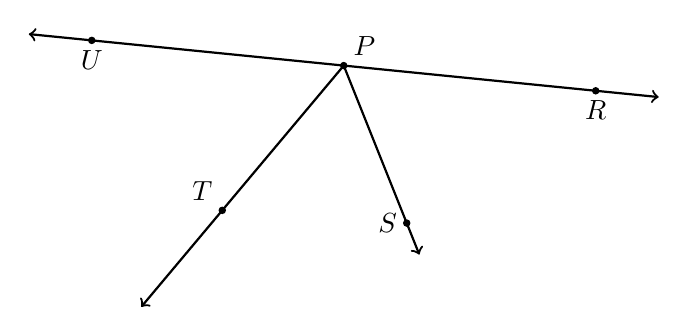
\begin{tikzpicture}[scale=0.8, rotate=180]
        \draw [->, thick] (0,0)--(50:5);
        \draw [<->, thick] (-5,.5)--(5,-.5);
        \draw [->, thick] (0,0)--(-1.2,3);
        \draw [fill] (-1,2.5) circle [radius=0.05] node[left ]{$S$};
        \draw [fill] (50:3) circle [radius=0.05] node[above left ]{$T$};
        \draw [fill] (0,0) circle [radius=0.05] node[above right]{$P$};
        \draw [fill] (4,-0.4) circle [radius=0.05] node[below]{$U$};
        \draw [fill] (-4,0.4) circle [radius=0.05] node[below]{$R$};
      \end{tikzpicture}
      \end{center}
    \begin{enumerate}
      \item True or False: $\overrightarrow{RP}$ and $\overrightarrow{UP}$ are opposite rays.\bigskip
      \item True or False: $\angle TPR$ is supplementary to $\angle TPU$.\bigskip
      \item True or False: $\angle RPS$ and $\angle TPS$ are complementary angles. \bigskip
      \item True or False: $\angle RPS$ and $\angle TPU$ are vertical angles. \bigskip
    \end{enumerate}

    \item The shape shown below is composed of straight lines and right angles, with some lengths as marked. Find the perimeter of the figure. Show your work.
    \begin{flushright}
    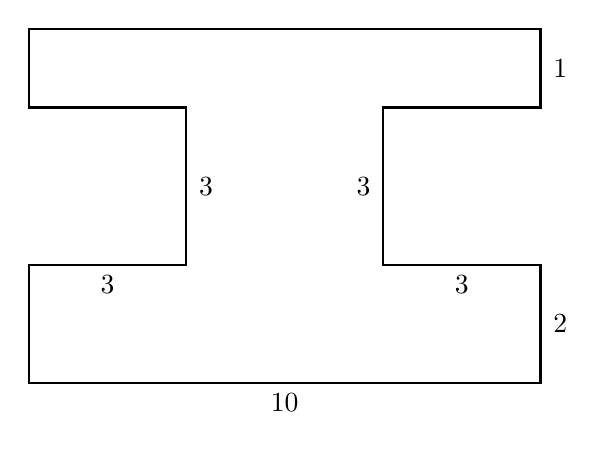
\begin{tikzpicture}[scale=0.5]
      \draw [-, thick] (0,0)--(13,0)--(13,3)--(9,3)--(9,7)--(13,7)--
      (13, 9)--(0,9)--(0,7)--(4,7)--(4,3)--(0,3)--cycle;
      %\draw [fill] (0,0) circle [radius=0.05] node[left]{$A$};
      %\draw [fill] (7,0) circle [radius=0.05] node[right]{$B$};
      %\draw [fill] (7,2) circle [radius=0.05] node[right]{$C$};
      %\draw [fill] (0,2) circle [radius=0.05] node[left]{$D$};
      \node at (4.5, 5){3};
      \node at (2, 2.5){3};
      \node at (8.5, 5){3};
      \node at (11, 2.5){3};
      \node at (6.5, -0.5){10};
      \node at (13.5, 1.5){2};
      \node at (13.5, 8){1};
    \end{tikzpicture}
    \end{flushright} 

\item Given $\overline{DEFG}$, $DE=1 \frac{2}{5}$, $EF=2 \frac{3}{10}$, and $FG= \frac{4}{5}$. (diagram not to scale)\\ [0.25cm]
  Find ${DG}$, expressed as a fraction, not a decimal.
  \begin{flushright}
      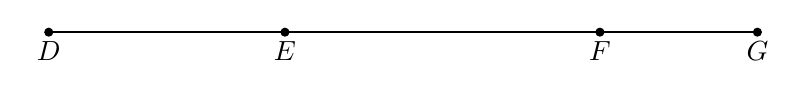
\begin{tikzpicture}
        \draw [-, thick] (0,0)--(9,0);
        \draw [fill] (0,0) circle [radius=0.05] node[below]{$D$};
        \draw [fill] (3,0) circle [radius=0.05] node[below]{$E$};
        \draw [fill] (7,0) circle [radius=0.05] node[below]{$F$};
        \draw [fill] (9,0) circle [radius=0.05] node[below]{$G$};
      \end{tikzpicture}
    \end{flushright}

\end{enumerate}
\end{document}
